%%%%%%%%%%%%%%%%%%%%%%%%%%%%%%%%%%%%%%%%%
% The Blabla Book
% Structural Definitions File
% Version 2.0 (9/2/15)
%
% Original author:
% lux.qc (lux.qc@yandex.com)
%
% CC BY-NC-SA 3.0 (http://creativecommons.org/licenses/by-nc-sa/3.0/)
%
%%%%%%%%%%%%%%%%%%%%%%%%%%%%%%%%%%%%%%%%%

%----------------------------------------------------------------------------------------
%	VARIOUS REQUIRED PACKAGES AND CONFIGURATIONS
%----------------------------------------------------------------------------------------

\usepackage[top=1.39cm,bottom=1.8cm,left=1.7cm,right=1.27cm,headsep=10pt,papersize={13.8cm ,21.6cm}
]{geometry}
\usepackage{indentfirst} 
\usepackage{graphicx} % Required for including pictures
\graphicspath{{Pictures/}}
\usepackage{tikz,pgfplots} % Required for drawing custom shapes
\pgfplotsset{compat=newest}
\usepackage{booktabs,enumerate} % Required for nicer horizontal rules in tables
\usepackage{xcolor} % Required for specifying colors by name
\definecolor{ocre}{RGB}{0,0,0} % Define the favorite color used for highlighting throughout the book
\bibliographystyle{alpha}


%----------------------------------------------------------------------------------------
%	PAGE HEADERS
%----------------------------------------------------------------------------------------

\usepackage{fancyhdr} % Required for header and footer configuration
%
%\pagestyle{fancy}
\renewcommand{\chaptermark}[1]{\markboth{\sffamily\normalsize\chaptername\ \thechapter.\ #1}{}} % Chapter text font settings
\renewcommand{\sectionmark}[1]{\markright{\normalfont\normalsize\thesection\hspace{5pt}#1}{}}


%----------------------------------------------------------------------------------------
%	CHINESE SETTING
%----------------------------------------------------------------------------------------
\usepackage[format=hang,labelfont=bf]{caption}
%\captionsetup{font={scriptsize}}
\captionsetup{figurename={图}, tablename={表}}
%\addto{\captionsenglish}{\renewcommand{\contentsname}{目\quad录}}
\def\chntoday{\the\year~年~\the\month~月~\the\day~日}
% adjust the width of tables to adapt it to the textwidth
\usepackage{tabularx}
\newcolumntype{Y}{>{\centering\arraybackslash}X} % New flag to centering the width-adapted columns

\usepackage{mathtools}
\usepackage[scr=boondoxo, scrscaled=1]{mathalfa}
%\usepackage{mathrsfs}
\usepackage{mathptmx,mathpazo}
\usepackage{old-arrows}
%\usepackage[T1]{fontenc}
%\usepackage{newpxtext,newpxmath}
%\usepackage{newtxtext}
%\usepackage{newtxmath,} %A systematic solution to Roamn font, including math font.
\usepackage{braket,ulem}
\renewcommand{\braket}[1]{\Braket{#1}}
\renewcommand{\ket}[1]{\Ket{#1}}
\renewcommand{\bra}[1]{\Bra{#1}}
%\usepackage[UTF8]{ctex}
\usepackage{luatexja-fontspec}
\setmainjfont{FandolSong}
\setsansjfont{FandolKai}

%\ctexset{fontset = none}
%\setmainfont{CMU Concrete}
\let\bar\undifined
\newcommand{\bar}[1]{\overline{#1}}
\newcommand{\scr}[1]{\mathscr{#1}}
\newcommand{\bo}[1]{\mathbf{#1}}
\renewcommand{\epsilon}{\varepsilon}
\newcommand{\sch}{Schr\"odinger}
\newcommand{\ha}{Hamiltonian}
%\newcommand{\dd}{\text{d}}
\usepackage{xparse}
\newcommand{\dd}[1]{\mathrm{d}\mathbf{#1}}
\let\dd\undefined
\NewDocumentCommand{\dd}{ g }{%
	\IfValueTF{#1}
	{% https://tex.stackexchange.com/q/53068/5764
		\if\relax\detokenize{#1}\relax
		\mathrm{d} %
		\else
		\mathrm{d}\mathbf{#1}%
		\fi}
	{\mathrm{d}}%
}
\newcommand{\ddx}{\dd\mathbf{x}}

\newcommand{\db}[1]{\dd\bo{#1}}
\newcommand{\hs}{\mathscr{H}}
\newcommand{\vs}{\mathscr{V}}
\newcommand{\es}{\mathscr{E}}
\renewcommand{\textit}[1]{\textgt{#1}}
\renewcommand{\itshape}{\jfontspec{FandolKai}}
\renewcommand{\emph}[1]{\textbf{#1}}


%\usepackage{chapterbib}

\usepackage{endnotes}
\renewcommand{\makeenmark}{\hbox{$^\theenmark$}}
\renewcommand{\notesname}{\bf 注释}
\makeatletter
\@addtoreset{endnote}{chapter}
\makeatother
%\let\footnote\endnote

%---------------------------------------------------------------------
% the command to generate two lines between which are the  excerise content, using amsthm to number the exercise.
\let\openbox\undefined
\usepackage{amsthm}
\newtheoremstyle{nx}{}{}{\normalfont}{}{\bfseries}{}{1em}{}
\theoremstyle{nx}
\newtheorem{Xercise}{$\qquad$练习}[chapter]
\newenvironment{xercise}{\par\vspace{\baselineskip}\noindent\hrule\vspace{.5\baselineskip}\Xercise}
{\vspace{\baselineskip}\hrule\par\endXercise}

\newcommand\Next{\endXercise\hrule\Xercise}
\newcommand{\exercise}[1]{\begin{xercise}#1\end{xercise}}
%========================================================

\newcommand{\tu}{\begin{figure}[h]
		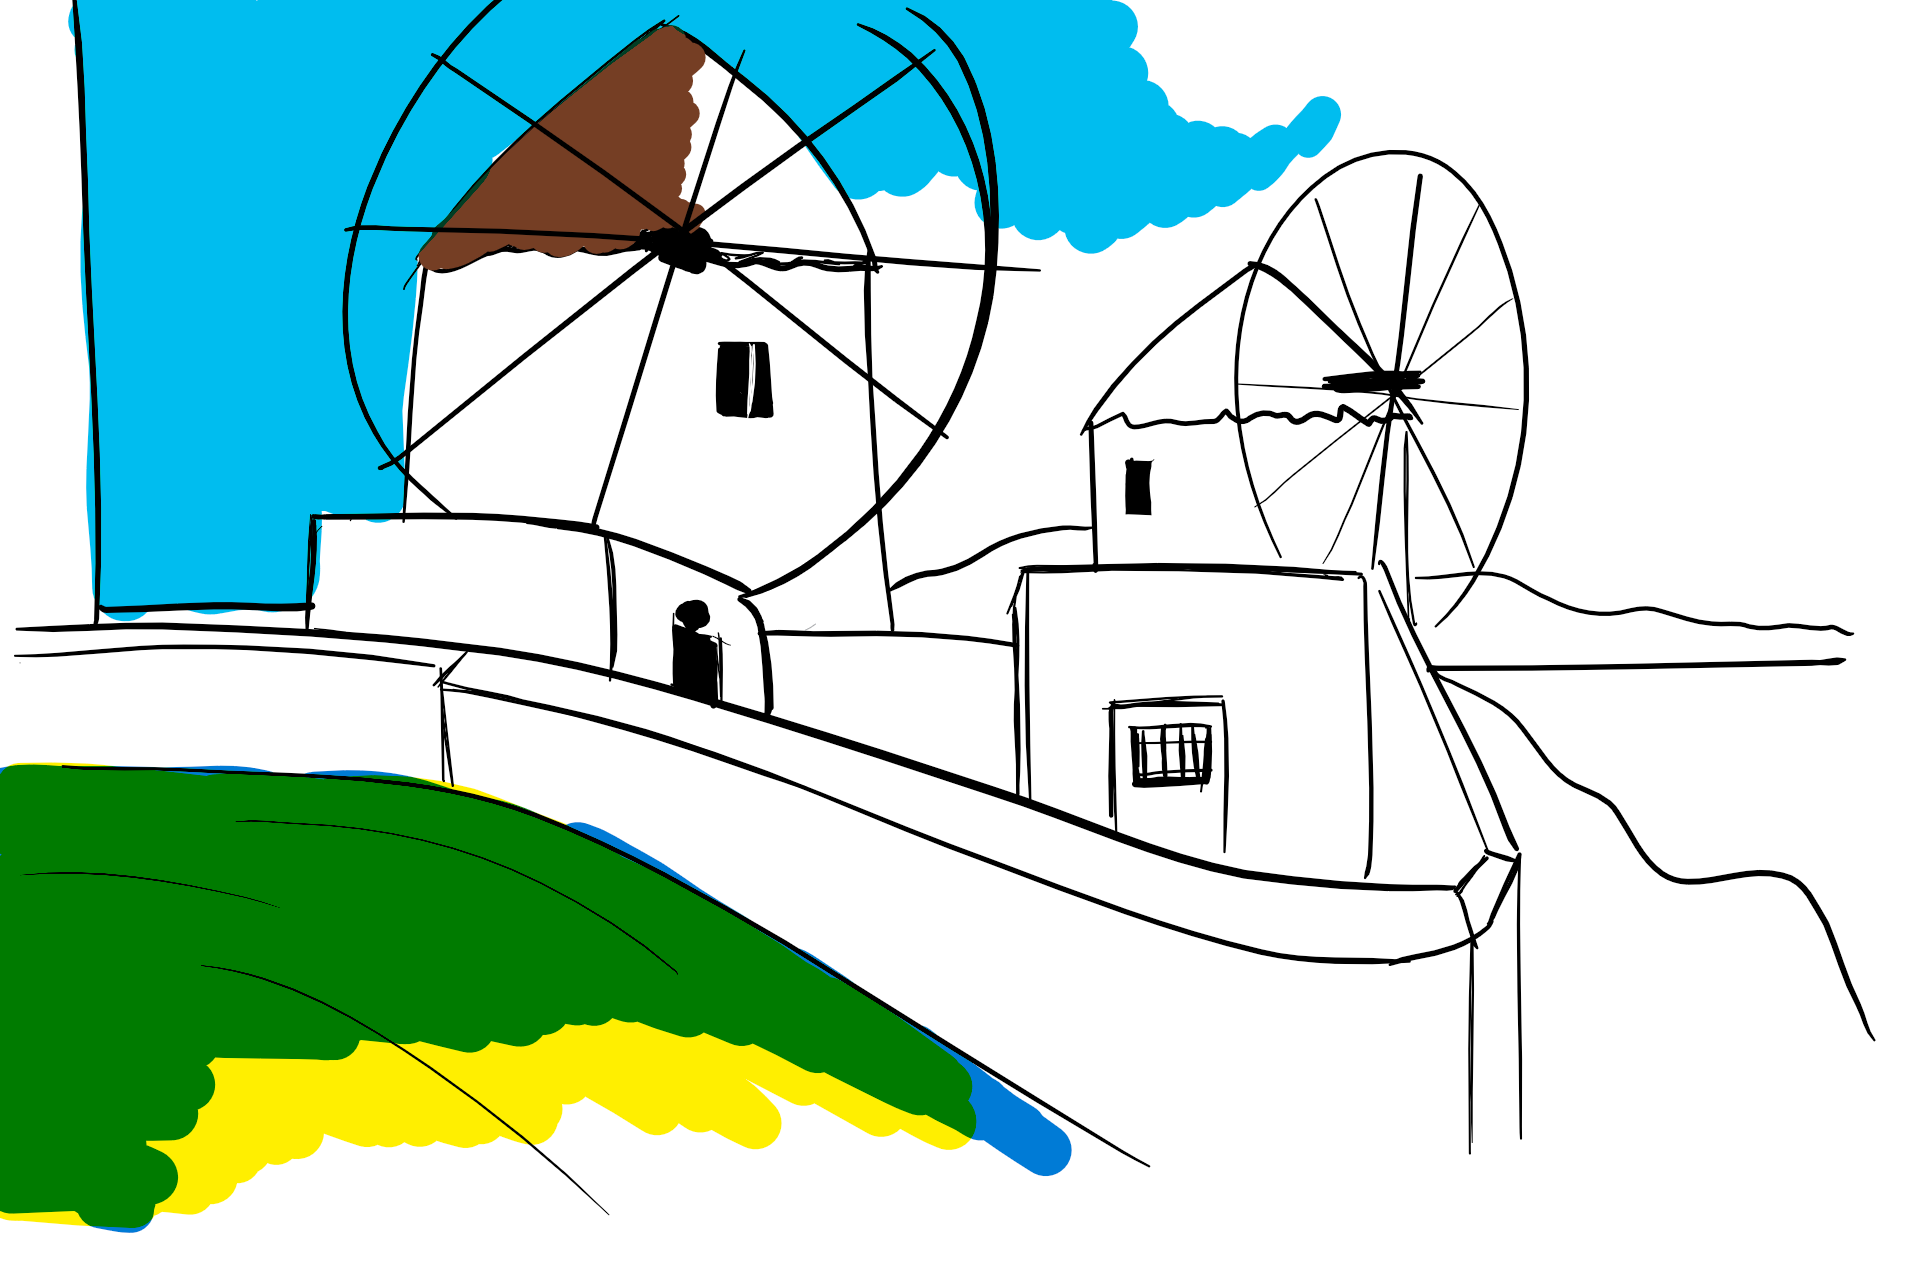
\includegraphics[width=.5\textwidth]{q.png}
\end{figure}}
% Feynman Diagram Setting
\usetikzlibrary{arrows.meta}
\newcommand{\midarrow}{\tikz \draw[-triangle 45] (0,0) -- +(.05,0);}
\tikzset{> = latex, color=blue}
\usetikzlibrary{decorations.markings,decorations.pathreplacing}
\tikzset{
	% style to apply some styles to each segment of a path
	on each segment/.style={draw=blue,
		decorate,
		    decoration={
			show path construction,
			moveto code={},
			lineto code={
				\path [#1]
				(\tikzinputsegmentfirst) -- (\tikzinputsegmentlast);
			},
			curveto code={
				\path [#1] (\tikzinputsegmentfirst)
				.. controls
				(\tikzinputsegmentsupporta) and (\tikzinputsegmentsupportb)
				..
				(\tikzinputsegmentlast);
			},
			closepath code={
				\path [#1]
				(\tikzinputsegmentfirst) -- (\tikzinputsegmentlast);
			},
		},
	},
	% style to add an arrow in the middle of a path
	mid arrow/.style={postaction={decorate,decoration={
				markings,
				mark=at position .55 with {\draw[arrows = {-Latex[width=0pt 7, length=5pt]}] (0pt,.0pt) -- (1.8pt,0pt);}
	}}},
	% style to add an reverse arrow in the middle of a path
	mid reverse arrow/.style={postaction={decorate,decoration={
			markings,
			mark=at position .45 with {\draw[arrows = {-Latex[width=0pt 7, length=5pt]}] (1.8pt,.0pt) -- (0pt,0pt);}
}}},
}
\newcommand{\dian}{\tikz{\filldraw[blue](0,0)circle(1pt)}}
\usepackage[compat=1.1.0]{tikz-feynman}
\usepackage{float}
\renewcommand{\normalsize}{\fontsize{8pt}{9.6pt}\selectfont}
\newcommand{\diagsize}{\fontsize{5pt}{6.6pt}\selectfont}
\newcommand{\cs}{a^\dagger}
\newcommand{\hd}{\mathrm{H}_2}
\newcommand{\hft}{Hartree-Fock}
\newcommand{\twoe}{r_{12}^{-1}}
\newcommand{\tp}{\tilde{\Phi}}
%\usepackage[symbol]{footmisc} 
\renewcommand{\thefootnote}{\roman{footnote}}
\newcommand{\bfr}{\mathbf{r}}
\newcommand{\heh}{\mathrm{HeH}^+}
% 注意core-hamitonian的替换, 正则->典则
\newcommand{\au}{\,\mathrm{a.u.}}
\usepackage{hyperref}